\subsection{Results analysis}

This section aim to understand : the errors of the system to try to solve them and to inspect the results to improve them.

\subsubsection{Distances' matrix visualization}

When computing the rank lists, each link have its distance calculated and can be represented in a matrix for the non-commutative distances functions and in a symmetric matrix for the commutative distances functions.
In this matrix each document represent a row and a column and the elements of the matrix to a link.
To visually represent the distances' matrix, each element of the matrix is mapped to a pixel in an 2D image.
The element value in the matrix is mapped to the pixel brightness, the low values are in light colours and high values in dark colours.
A good distance matrix should have each same author documents pair with a low distances (light colour in the image) and different authors documents pairs with a high distance (dark colour in the image).
The greater the contrast between the true links (same author documents) and the false links (different authors documents) is, the better the text representation is, since the related rank list will have a greater average precision.
When the documents are sorted alphabetically by their authors and if the distances' matrix can represent correctly the author style, same authors documents have generally a low distance, this creates light colour squares in the diagonal.
The square size is related to the number of document written by this author.
The diagonal is the lightest colour (white), since the distance between two same documents is always 0, with respect to the identity of indiscernible axiom of the distance functions.

The distance matrix for the best retained representation (the highest average precision) and the worse retained text representation (the lowest average precision) is visually presented in Figure~\ref{fig:distances_matrix_oxquarry} for Oxquarry.
Respectively the Clark distance on the $750$-MFW which gives an average precision of $0.89$, and the Tanimito distance on the $750$-MFW gives an $0.63$ average precision.
The diagonal is white in both images, a light colour square in the diagonal can clearly be observed on both distance matrix visualizations, even thought some are slightly tainted.
Clark has overall a good distances matrix, except some document pairs from Conrad, Hardy and Orczy which have darker colours, these are ranked below some false links in the rank list.
For Tanimoto, firstly one can observe these stripes, which are due to the max function in its computation, which create more cleaved decision in the score value.
The main suspects for this observation is probably due to some high frequency term only used in some excerpts, thus when normalizing by the sum of maxima in the Tanimoto computation, document with these high relative frequency create these stripes.

\begin{figure}
  \caption{Distance matrix visualization Oxquarry}
  \label{fig:distances_matrix_oxquarry}

  \caption{Best retained text representation for Oxquarry ($750$-MFW tokens with Clark)}
  \label{fig:distance_matrix_oxquarry_clark}
  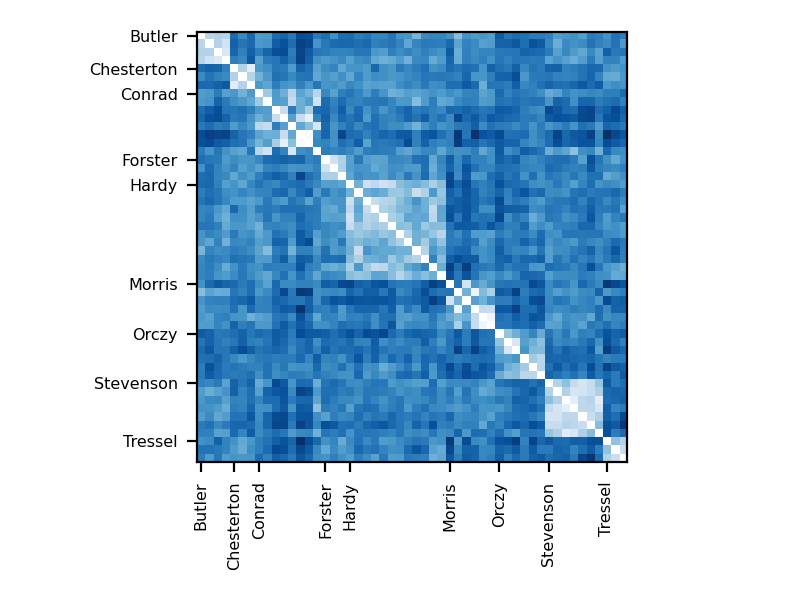
\includegraphics{img/distance_matrix_oxquarry_clark.png}

  \caption{Worse retained text representation for Oxquarry ($750$-MFW tokens with Tanimoto)}
  \label{fig:distance_matrix_oxquarry_tanimoto}
  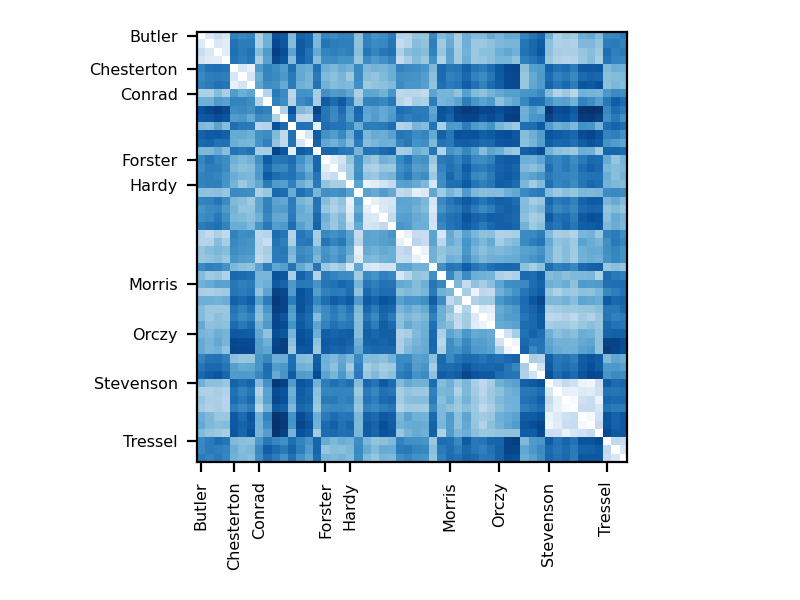
\includegraphics{img/distance_matrix_oxquarry_tanimoto.png}
\end{figure}

\subsubsection{Links scores distribution in rank lists}

In Savoy (2014)'s \textit{Estimating the Probability of an Authorship Attribution} they modelized the distribution of the true and false links across the score obtained using a mixture of 2 beta distribution.
Using the 2 beta distribution models an approximation of the probability of being a true link can be computed using the following formula.

Figure~\ref{fig:links_score_density} show the density of true and false link as well as a beta distribution estimation for St-Jean (Regression fusion in \ref{fig:links_score_density_fusion_regression} and Z-Score fusion in \ref{fig:links_score_density_fusion_z_score}).
For the Z-score fusion, the distances have been normalized between 0 and 1 using Definition~\ref{def:normalization} to be able to estimate the beta distribution.

The results obtained by the regression fusion already are a probability of being a true link so the use of the beta distribution is limited, the two distribution are already well seperated.
In the other hand, for the z-score fusion, it is possible to hestimate the probability of being a true link using the area under the curve of the two beta distribution.
The vectical line indicate the postion where both beta distribution have the same probability of being a true link and false link (same area under the curve).
This point can be used as alternative decision point where the cut should be made in the rank list, this ensure that both false positives and false negatives are minimized.

\begin{figure}
  \caption{Links score distribution and beta distribution estimation for St-Jean}
  \label{fig:links_score_density}

  \subcaption{Regression fusion (training Oxquarry)}
  \label{fig:links_score_density_fusion_regression}
  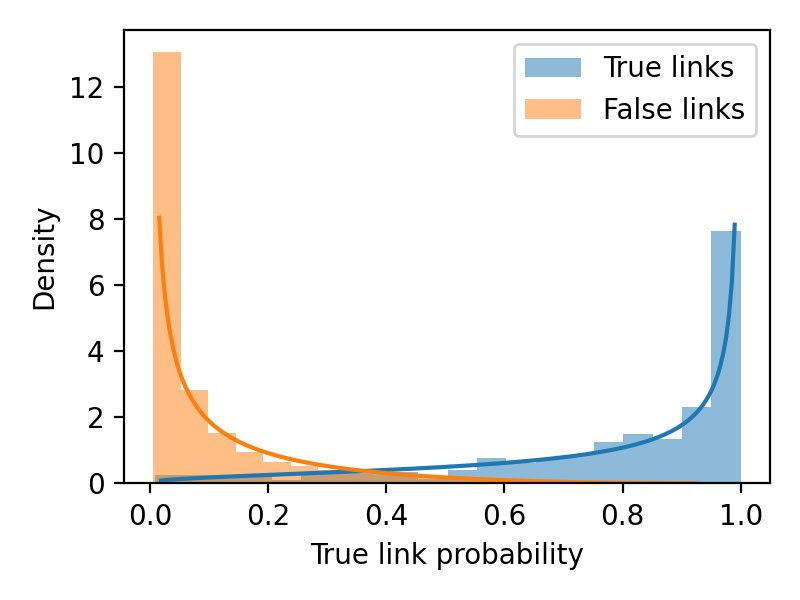
\includegraphics[width=\linewidth]{img/links_score_density_fusion_regression.png}

  \subcaption{Z-Score fusion}
  \label{fig:links_score_density_fusion_z_score}
  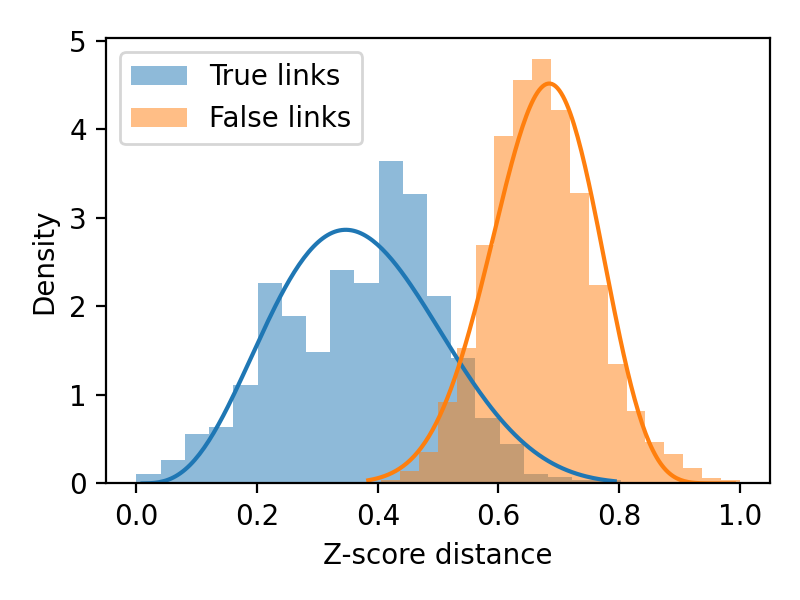
\includegraphics[width=\linewidth]{img/links_score_density_fusion_z_score.png}
\end{figure}

\subsubsection{Frequent errors}
\label{sec:frequent_errors}

For this experiment, the goal is to try to understand the errors in the system, in this case the false links (document pairs with different authors) highly ranked on different rank lists.
The rank list quality is high based on the text representation and the distance function, but mostly on the first.
The previous statement can be deduced by the following reasoning : For example when using the $n$-MFW method, if two documents feature vector are closely related (nearly identical), no matter the distance function they should have a low distance, since every distance function should give a distance of 0 when computing the distance between two identical vectors.
We believe some errors in the system are due to documents having close feature vectors values even though they are not from the same authors.
To motivate this statement the following experiment is realized.

The 4 token-based retained rank list from the St-Jean corpus are used, see Table~\ref{tab:9rl_results_st_jean_A_B} in annex.
These 4 rank lists are using the same text representation, in this case the relative frequency of the $750$-MFW tokens as feature vector, only the distance function used to create the rank list is different.
The goal is to compare the feature vector of the two documents for some specific link, in our case the following were chosen : Frequent errors, ranked first in a rank list (most similar vectors, according to the distance function), ranked last in a rank list (the least similar vectors) and Ranked HPrec-th in a rank list.
Links often appearing in the top 20 false links in all 4 rank lists are considered as frequent errors.
The rank list used for the comparison is the one with the best average precision, in this case the one using Manhattan distance, with an average precision of 0.78.
To perform a comparison, a visualization of the feature vector is done using a bar plot.
In this case, the visualization is based on the $750$-MFW tokens representation, since the rank lists were created using this vector size.
To be able to understand more easily this vector, the values have been sorted by the mean relative frequencies and use a logarithmic scale.
When a large proportion of the vectors overlap it indicates a high similarity between the MFW vectors.
Both document style are close when their feature vector are closely related.
Visually when most of the surface overlap, the distance function will give a low value, and with a correct distance measure should be ranked high in the list.

Figures~\ref{fig:mfw_vector_error} show the feature vector of two frequent errors document pairs (document 48 from Vigny / document 62 from Dumas and document 10 from Maupassant / document 52 from Flaubert), these link appear in the top 20 false links of 3 out 4 rank lists.
The frequent errors vector pairs presented in Figure~\ref{fig:mfw_vector_error} can be visually compared actual true links and actual false links, to have a better understanding of this problematic.
For example the most similar true link (ranked 1 using Manhattan distance) in Figure~\ref{fig:mfw_vector_first_rl} (documents 30 and 116 from Sand) or the HPrec-th (last continuous correct pair from the top of the list) in Figure~\ref{fig:mfw_vector_first_last_rl} (documents 184 and 192 from Barbey), both of these links show a large proportion of overlapping surface, like for the frequent errors vectors.
A counter example would be the least similar false link (ranked last using Manhattan distance) which represent a negatively correlated document pair, Figure~\ref{fig:mfw_vector_last_rl} showcase this link (document 183 from Stael / document 194 from Regnier).
As expected, most of this figure surface is non-overlapping.

When two vectors are relatively close together, determining that two texts are from a different author can not clearly be established using only one type of representation, no matter the distance metric applied.
Thus, this experiment showcase the need of having multiple text representation to obtain more robust solutions.

\begin{figure}
  \centering
  \caption{Example of 750-MFW relative frequency vectors for the two documents in a reccurant false link in the top 20 false links}
  \label{fig:mfw_vector_error}

  \subcaption{First example}
  \label{fig:mfw_vector_error_0}
  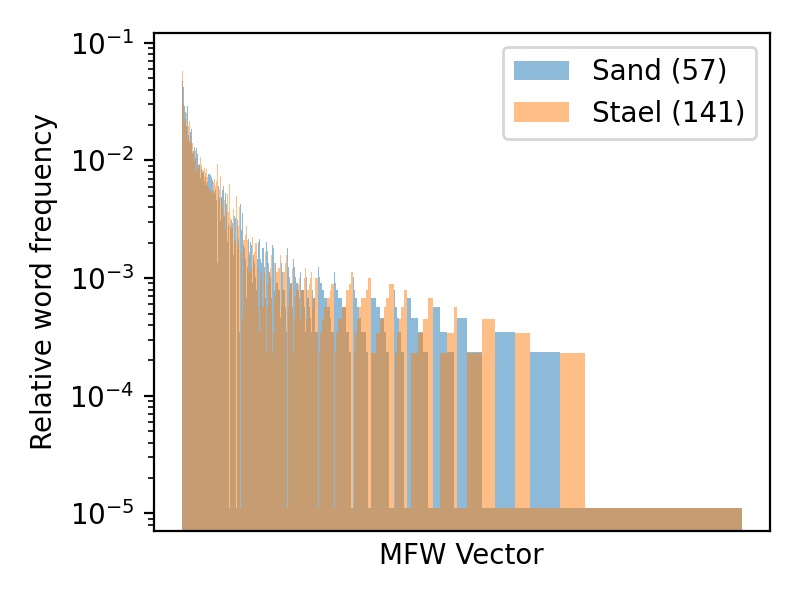
\includegraphics[width=\linewidth]{img/mfw_vector_error_0.png}

  \subcaption{Second example}
  \label{fig:mfw_vector_error_1}
  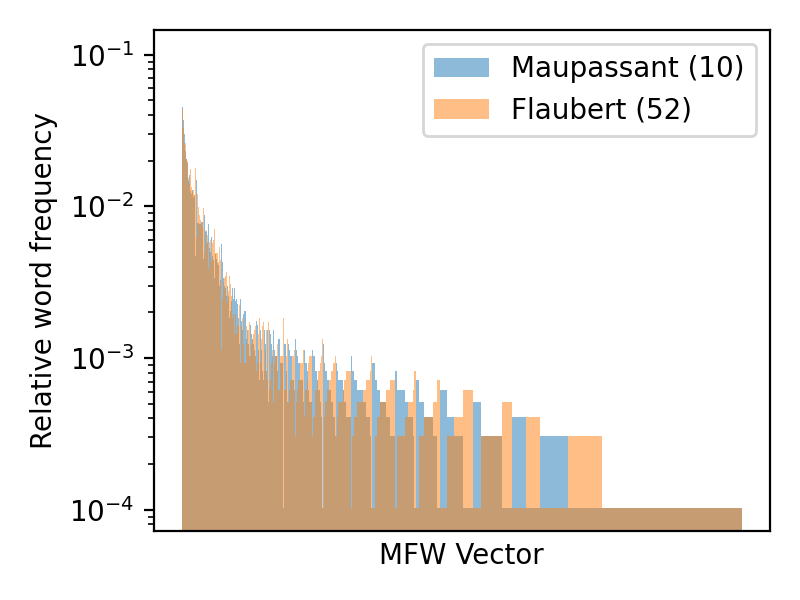
\includegraphics[width=\linewidth]{img/mfw_vector_error_1.png}
\end{figure}

\begin{figure}
  \centering
  \caption{750-MFW relative frequency for the two documents ranked $X$ in the rank list using the token representation on St-Jean}

  \subcaption{$X$ = First}
  \label{fig:mfw_vector_first_rl}
  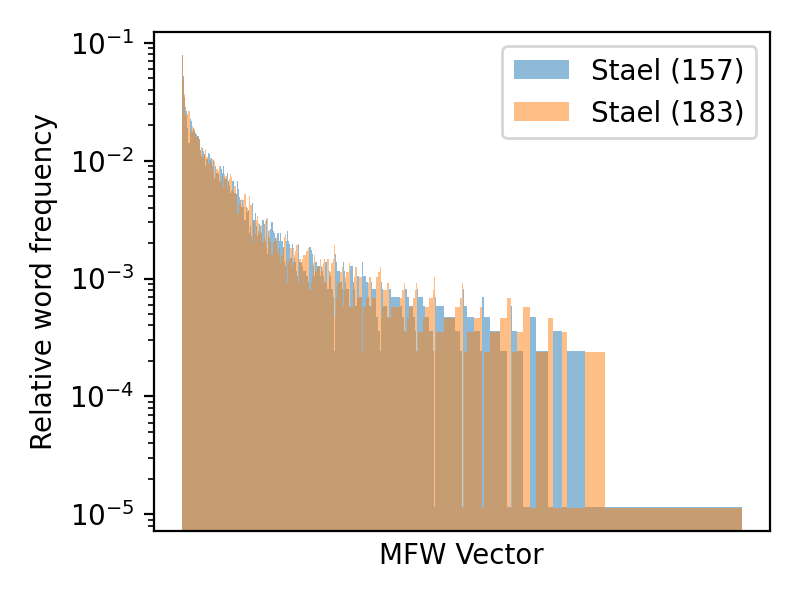
\includegraphics[width=\linewidth]{img/mfw_vector_first_rl.png}

  \subcaption{$X$ = HPrec-th}
  \label{fig:mfw_vector_first_last_rl}
  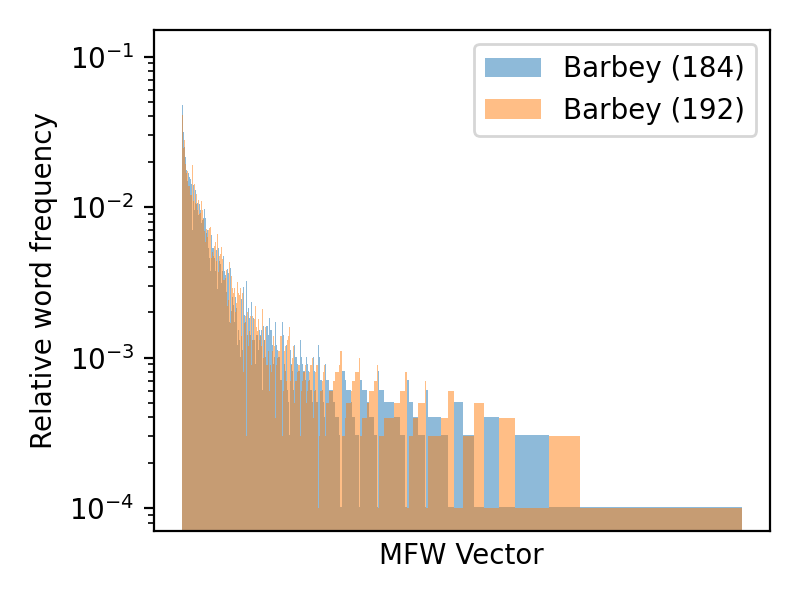
\includegraphics[width=\linewidth]{img/mfw_vector_first_last_rl.png}

  \subcaption{$X$ = Last}
  \label{fig:mfw_vector_last_rl}
  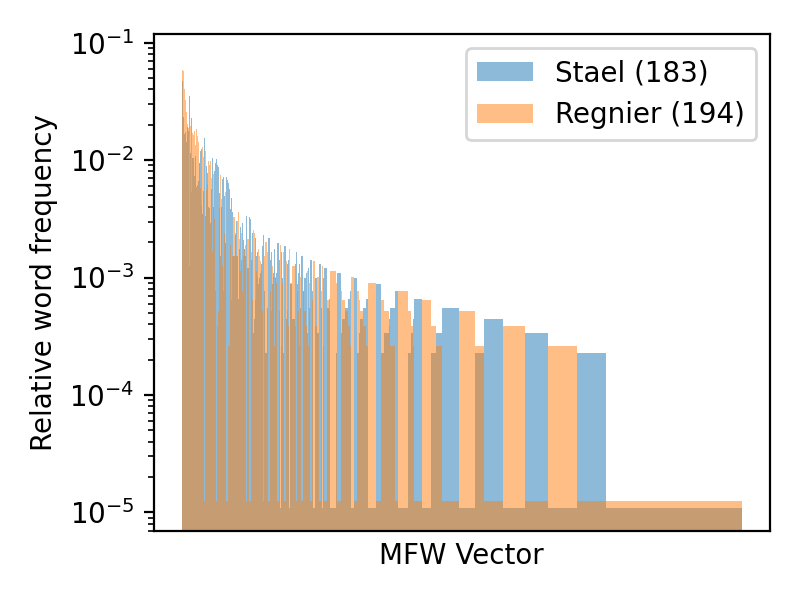
\includegraphics[width=\linewidth]{img/mfw_vector_last_rl.png}
\end{figure}

\subsubsection{Publication date differences analysis}

When dealing with false links ranked high in the rank list, as the previous experiment showed, some excerpt use similar words.
These shared words might be related to the era the book was written in.
The following experiment try to investigate on this by analysing the difference in publication date for the most incorrect document pairs in the rank lists (false links ranked high in the rank list).

In the St-Jean corpus publication paper, the publication dates of each excerpts are available~\cite{st_jean}.
First the publication date distribution of the corpus must be understood, to further continue the experiment.
Figure~\ref{fig:dates_distribution} show the distribution of the publication date in the St-Jean corpus.
The corpus mainly focus on the two last thirds of the XIX century, only a few books are published between 1800 and 1830.
The date difference distribution for each pair of documents can be computed, Figure~\ref{fig:dates_differences_true_false} shows the date difference distribution for the true and false links.
The union of both of them represent every possible document pairs (the whole rank list), in this Figure the bars are stacked to represent every link.
Table~\ref{tab:date_differences} show statistics on the distributions.
True links have a low mean date difference of 5.11 years with a standard deviation of 7.05.
The low mean can be explained by the fact that most authors in St-Jean have excerpts from the same book and the authors publish their books during their career, which is limited to their active years (life span minus early stages and old age for most authors).
In fact, 281 of the 670 ($\sim 42\%$) true links were published the same year and 453 out of 670 ($\sim 68\%$) true links have a publication date difference below or equal to 5 years.
For St-Jean the largest date difference from the same author (correspond to the longest career) is 31 years, which correspond to the two following books  from Victor Hugo : \textit{Notre Dame de Paris} (The Hunchback of Notre-Dame), in 1831 and \textit{Les Misérables}, in 1862.
The average date difference for the false links is 28.24 years with a standard deviation of 20.73 years.
The overall average (both true and false links) is at 29.04 years with a standard deviation of 20.58.

The previous statistics can be compared to the ones in Figure~\ref{fig:dates_differences_r_false} which show the date difference density on the top-r false links (top-670 in case of St-Jean) on a rank list with 85\% average precision (z-score fusion of the retained text representations, Table~\ref{tab:9rl_results_st_jean_A_B}).
Two interesting information can be extracted here.
First the mean is lower by 7.75 years (29.04 - 21.29) compared to every false links and have a narrow standard deviation distribution.
Having a lower mean in this case indicate that more mistakes are made for document pairs with a lower date difference then for the ones with a large date difference, which can lead to the following conclusion : distinguishing between a false link and a true link for documents pair with low date difference is harder.
Secondly, we can observe a drop after 35 years of date difference, which indicate that links in the interval $\left[0-35\right]$ years are harder to discriminate between a true link and a false link than links outside this interval.
This 35 years interval can be related to the generation factor, the age of woman giving birth is around 25-34 in France~\cite{generations}, authors birth country in this corpus.
Each new generation tend to use its own vocabulary, and thus it can be harder to discriminate the author of text belonging to the same generation, if we assume that the authors write their books at around the same age.
In the other hand, having different vocabulary can indicate a different time period and is often used to detect document forgery~\cite{savoy_stylo}.
The small spike between 60 and 65 in the top-r false link is due to the matching of most excerpts from \textit{Volupté} (excerpts 117, 135, 151, 165, 181, 189) written by Charles Sainte-Beuve in 1834 and \textit{Les plaisirs et les jours} (excerpts 114, 132, 148) written by Marcel Proust in 1896.
Out of the 18 possible false link for these excerpts, 12 are in the top-r false link, which indicate that the styles used in these excerpts are close and can't discriminate the authors correctly even though the books were published with 62 years interval.

\begin{figure}
  \centering
  \caption{Dates distribution and date differences distribution on St-Jean}

  \subcaption{Dates distribution}
  \label{fig:dates_distribution}
  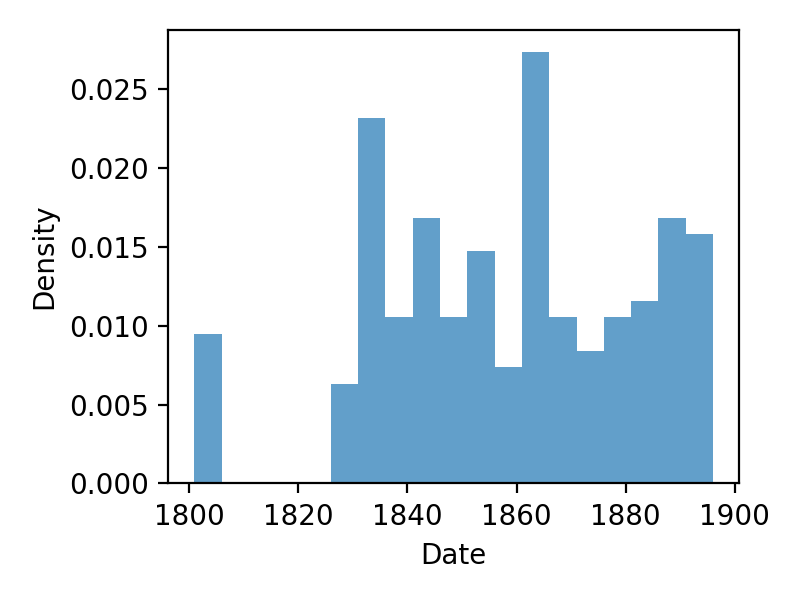
\includegraphics[width=\linewidth]{img/dates_distribution.png}

  \subcaption{True and false links date differences distribution}
  \label{fig:dates_differences_true_false}
  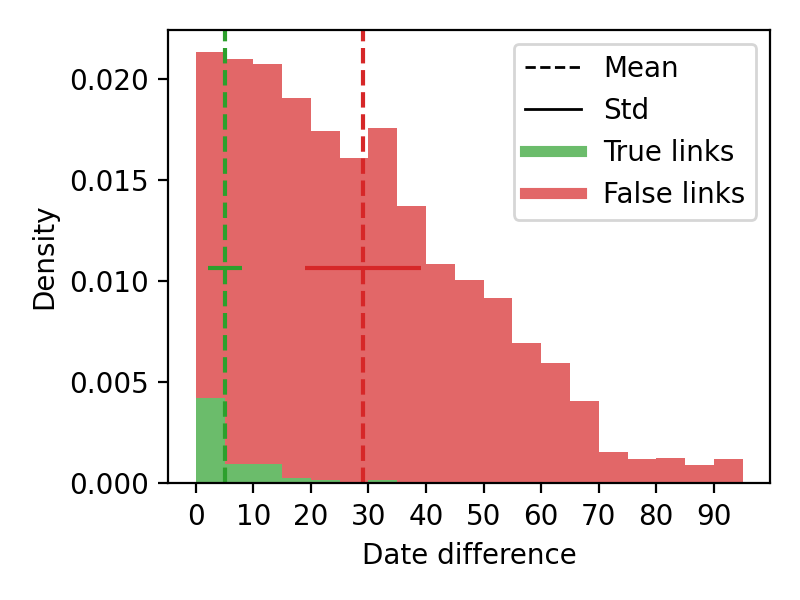
\includegraphics[width=\linewidth]{img/dates_differences_true_false.png}

  \subcaption{Top-r false links using a rank list with 85\% average precision}
  \label{fig:dates_differences_r_false}
  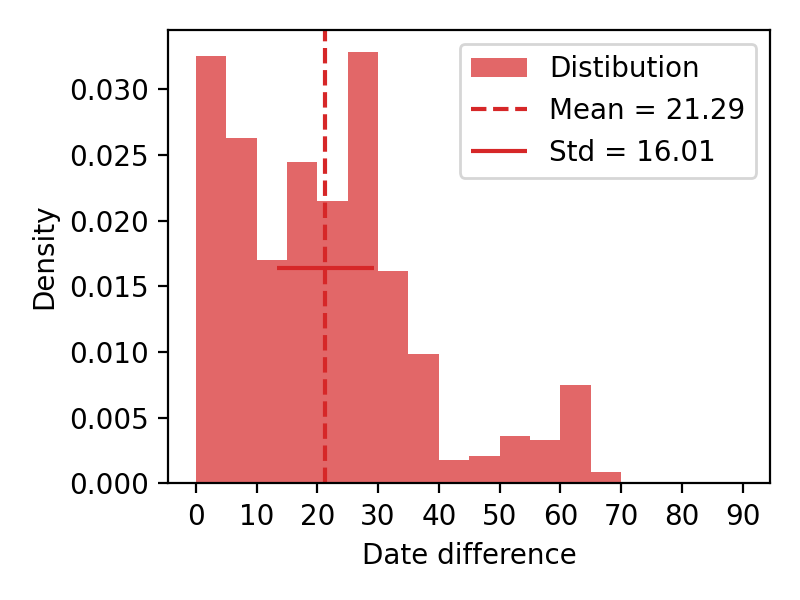
\includegraphics[width=\linewidth]{img/dates_differences_r_false.png}
\end{figure}

\begin{table}
  \centering
  \caption{Date differences statistics}
  \label{tab:date_differences}
    \begin{tabular}{l r r}
      \toprule
      Links                & Mean  & Std   \\
      \midrule
      True links           &  5.11 &  7.06 \\
      False links          & 29.04 & 20.58 \\
      True and False links & 28.24 & 20.73 \\
      top-r False links    & 21.29 & 16.00 \\
      \bottomrule
    \end{tabular}
\end{table}
